\documentclass[SE,lsstdraft,authoryear,toc]{lsstdoc}
\input{meta}

% Package imports go here.

\usepackage{tabularx,array}

% Local commands go here.


\title{Investigation of Ellipticity as a Function of the Degrees of Freedom}

% This can write metadata into the PDF.
% Update keywords and author information as necessary.
\hypersetup{
    pdftitle={Ellipticity_DOFs},
    pdfauthor={RebekahPolen},
    pdfkeywords={}
}

\input{authors}

\setDocRef{SOTN-003}
\setDocUpstreamLocation{\url{https://github.com/lsst-so/sotn-003}}

\date{\vcsDate}

\setDocAbstract{%\

% with short title this is only visible in the side-bar, so pare it down

This technote outlines the investigation into a potential relationship between ellipticity across the focal plane of the LSST Camera and the degrees of freedom of the Simonyi Survey Telescope. 
Such a finding would allow us to manipulate the optical system in order to correct for ellipticity when the behavior is contributing to the degradation of the point spread function. 
The results of this investigation reveal that, likely due to the nonlinear nature of second moments and ellipticity, any relationship to the degrees of freedom cannot be established. 
Rather, the investigation implies that the common assumption that the degrees of freedom originate near zero is usually false. 

% original abstract 

%This technote outlines the investigation into a potential relationship between ellipticity across the focal plane of the LSST Camera and the degrees of freedom of the Simonyi Survey Telescope. 
%The aim of this investigation was ideally to find a relationship between the behavior of the ellipticity and a particular degree of freedom or combination of degrees of freedom. 
%Such a finding would allow us to manipulate the optical system in order to correct for ellipticity when the behavior is contributing to the degradation of the point spread function. 
%The results of this investigation reveal that, likely due to the nonlinear nature of second moments and ellipticity, any relationship to the degrees of freedom cannot be established. 
%Rather, the investigation implies that the common assumption that the degrees of freedom originate near zero is usually false. 
%Without knowing the initial conditions of the optical system, it becomes difficult to infer any potential relationship to the ellipticity behavior. 
%Ultimately, this investigation suggests that standing assumption that the initial conditions for the optical system being approximately zero is not reliable. 


}

% Change history defined here.
% Order: oldest first.
% Fields: VERSION, DATE, DESCRIPTION, OWNER NAME.
% See LPM-51 for version number policy.
\setDocChangeRecord{%
  \addtohist{1}{YYYY-MM-DD}{Unreleased.}{Polen}
}


\begin{document}


%\maketitle
\mkshorttitle  %for technotes, remove extra pages

\section{Introduction}

The Vera C. Rubin Observatory Active Optics System (AOS) relies on curvature wavefront sensing to measure and correct for offsets on the Simonyi Survey Telescope \cite{Xin2015}. 
The AOS does this by manipulating the 50 degrees of freedom of the optical components of the telescope: the LSST Camera, the M2 secondary mirror, and the M1M3 mirror monolith consisting of the primary and tertiary mirrors. 
By ensuring that the optical components of the telescope are optimally aligned, we can improve image quality and reduce optical contributions to the point spread function (PSF). 

However, the ellipticity across the focal plane has been less responsive to AOS efforts to correct misalignment on the telescope. 
Ellipticity is defined as the amount of deviation from a perfect circle or sphere. 
On a telescope, ellipticity is measured from the components of the second-moment matrix:

\begin{equation}
    I = \begin{bmatrix} I_{xx} & I_{xy} \\ I_{yx} & I_{yy} \end{bmatrix}
\end{equation}

in which $I$ is calculated from the image intensity about the centroid. 
The ellipticity values $e_{1}$ and $e_{2}$ for the focal plane are then calculated from these matrix components:

\begin{equation}
    e_{1} = \frac{I_{xx}-I_{yy}}{I_{xx}+I_{yy}}
\end{equation}

and

\begin{equation}
    e_{2} = \frac{2 I_{xy}}{I_{xx}+I_{yy}}
\end{equation}

where $e_{1}$ is the ellipticity along the x- and y-axes and $e_{2}$ is the ellipticity along the axes rotated by 45$^{\circ}$. 
Both of these values are measured and reported to Rubin TV per in-focus exposure, as well as ingested in the \texttt{ConsDB}.

A coherent ellipticity pattern across the focal plane is dominated by effects originating from the optical system itself \cite{Jarvis2008}. 
However, this is less likely to be corrected by the AOS compared to other typical optical aberrations represented by the Zernike polynomials since they share a linear relationship to the total wavefront error. 
Ellipticity, on the other hand, is represented by second moments. 
Changing one Zernike value will linearly add or take away from the total wavefront error, while any change to the intensity distribution will change the second moments globally across the image. 
Despite this more complex relationship, the goal of these observations was to be able to identify a correlation visually between the ellipticity and degrees of freedom and use this as a starting point to better understand the relationship.  

\section{Observation Methods}

Data for this investigation was taken intermittently on the Rubin Observatory from April to September of 2025.
For each observation, a degree of freedom was selected and perturbed by a large amount, either in degrees or microns depending on the index.
After perturbing the selected degree of freedom, a set of 5 triplets were taken in series with either a 15 or 30 second exposure time.
The set of 5 triplets allowed us to average over the exposures to reduce the atmospheric effects and see any expected ellipticity patterns more clearly.
The offsets applied to the selected degrees of freedom are listed in Table \ref{tab:perturbations}.
In total, the data for this investigation is comprised of 117 exposures. 

\begin{table*}
\centering
\caption{This table is an outline of all the perturbations applied to the degrees of freedom of the telescope. For perturbations to the bending modes or $x$, $y$, and $z$ components of the hexapods, the units are in microns. For perturbations to the hexapod tilts ($rx$ or $ry$) the units are in degrees.}
\vspace{4pt}
\label{tab:perturbations}

\begin{tabularx}{\textwidth}{|>{\centering\arraybackslash}X|
                              >{\centering\arraybackslash}X|
                              >{\centering\arraybackslash}X|
                              >{\centering\arraybackslash}X|}
\hline
\textbf{Cam \textit{z}} & -75.0 & \textbf{M1M3 B16} & -0.03125 \\
\hline
\textbf{Cam \textit{x}} & -2000.0, -2500.0 & \textbf{M1M3 B17} & -0.05 \\
\hline
\textbf{Cam \textit{y}} & -2000.0, -2500.0 & \textbf{M1M3 B18} & -0.05 \\
\hline
\textbf{Cam \textit{rx}} & -0.01, -0.05 & \textbf{M1M3 B19} & -0.0375 \\
\hline
\textbf{Cam \textit{ry}} & -0.01, -0.05 & \textbf{M1M3 B20} & -0.025 \\
\hline
\textbf{M2 \textit{z}} & -75.0 & \textbf{M2 B1} & -0.3, -0.5 \\
\hline
\textbf{M2 \textit{x}} & -2000.0 & \textbf{M2 B2} & -0.5 \\
\hline
\textbf{M2 \textit{y}} & -2000.0 & \textbf{M2 B3} & -0.5 \\
\hline
\textbf{M2 \textit{rx}} & -0.01 & \textbf{M2 B4} & -0.5 \\
\hline
\textbf{M2 \textit{ry}} & -0.01 & \textbf{M2 B5} & -0.25 \\
\hline
\textbf{M1M3 B1} & -0.5 & \textbf{M2 B6} & -0.5 \\
\hline
\textbf{M1M3 B2} & -0.5 & \textbf{M2 B7} & -0.5 \\
\hline
\textbf{M1M3 B3} & -0.5 & \textbf{M2 B8} & -0.25 \\
\hline
\textbf{M1M3 B4} & -0.375 & \textbf{M2 B9} & -0.25 \\
\hline
\textbf{M1M3 B5} & -0.375 & \textbf{M2 B10} & -0.25 \\
\hline
\textbf{M1M3 B6} & -0.5 & \textbf{M2 B11} & -0.25 \\
\hline
\textbf{M1M3 B7} & -0.5 & \textbf{M2 B12} & -0.25 \\
\hline
\textbf{M1M3 B8} & -0.25 & \textbf{M2 B13} & -0.25 \\
\hline
\textbf{M1M3 B9} & -0.25 & \textbf{M2 B14} & -0.2 \\
\hline
\textbf{M1M3 B10} & -0.25 & \textbf{M2 B15} & -0.075 \\
\hline
\textbf{M1M3 B11} & -0.25 & \textbf{M2 B16} & -0.075 \\
\hline
\textbf{M1M3 B12} & -0.1875 & \textbf{M2 B17} & -0.075 \\
\hline
\textbf{M1M3 B13} & N/A & \textbf{M2 B18} & -0.025 \\
\hline
\textbf{M1M3 B14} & -0.05 & \textbf{M2 B19} & -0.025 \\
\hline
\textbf{M1M3 B15} & -0.0625 & \textbf{M2 B20} & -0.025 \\
\hline
\end{tabularx}
\end{table*}

\section{Analysis}

In order to analyze this data, we compared the on-sky images to models created using \texttt{StarSharp}: a simulation package which allowed us to simulate the focal plane based on input perturbations to any of the degrees of freedom. 
For each on-sky exposure, a corresponding model image was built with \texttt{StarSharp} to compare the expected patterns for particular bending mode. 
Expected patterns for each of the bending mode degrees of freedom can also be seen in Figures 1 and 2 of \cite{bending_modes}.
Below, Figure \ref{fig:example_image} shows derived on-sky second moment data next to the \texttt{StarSharp} model for this investigation.

\begin{figure}
    \centering
    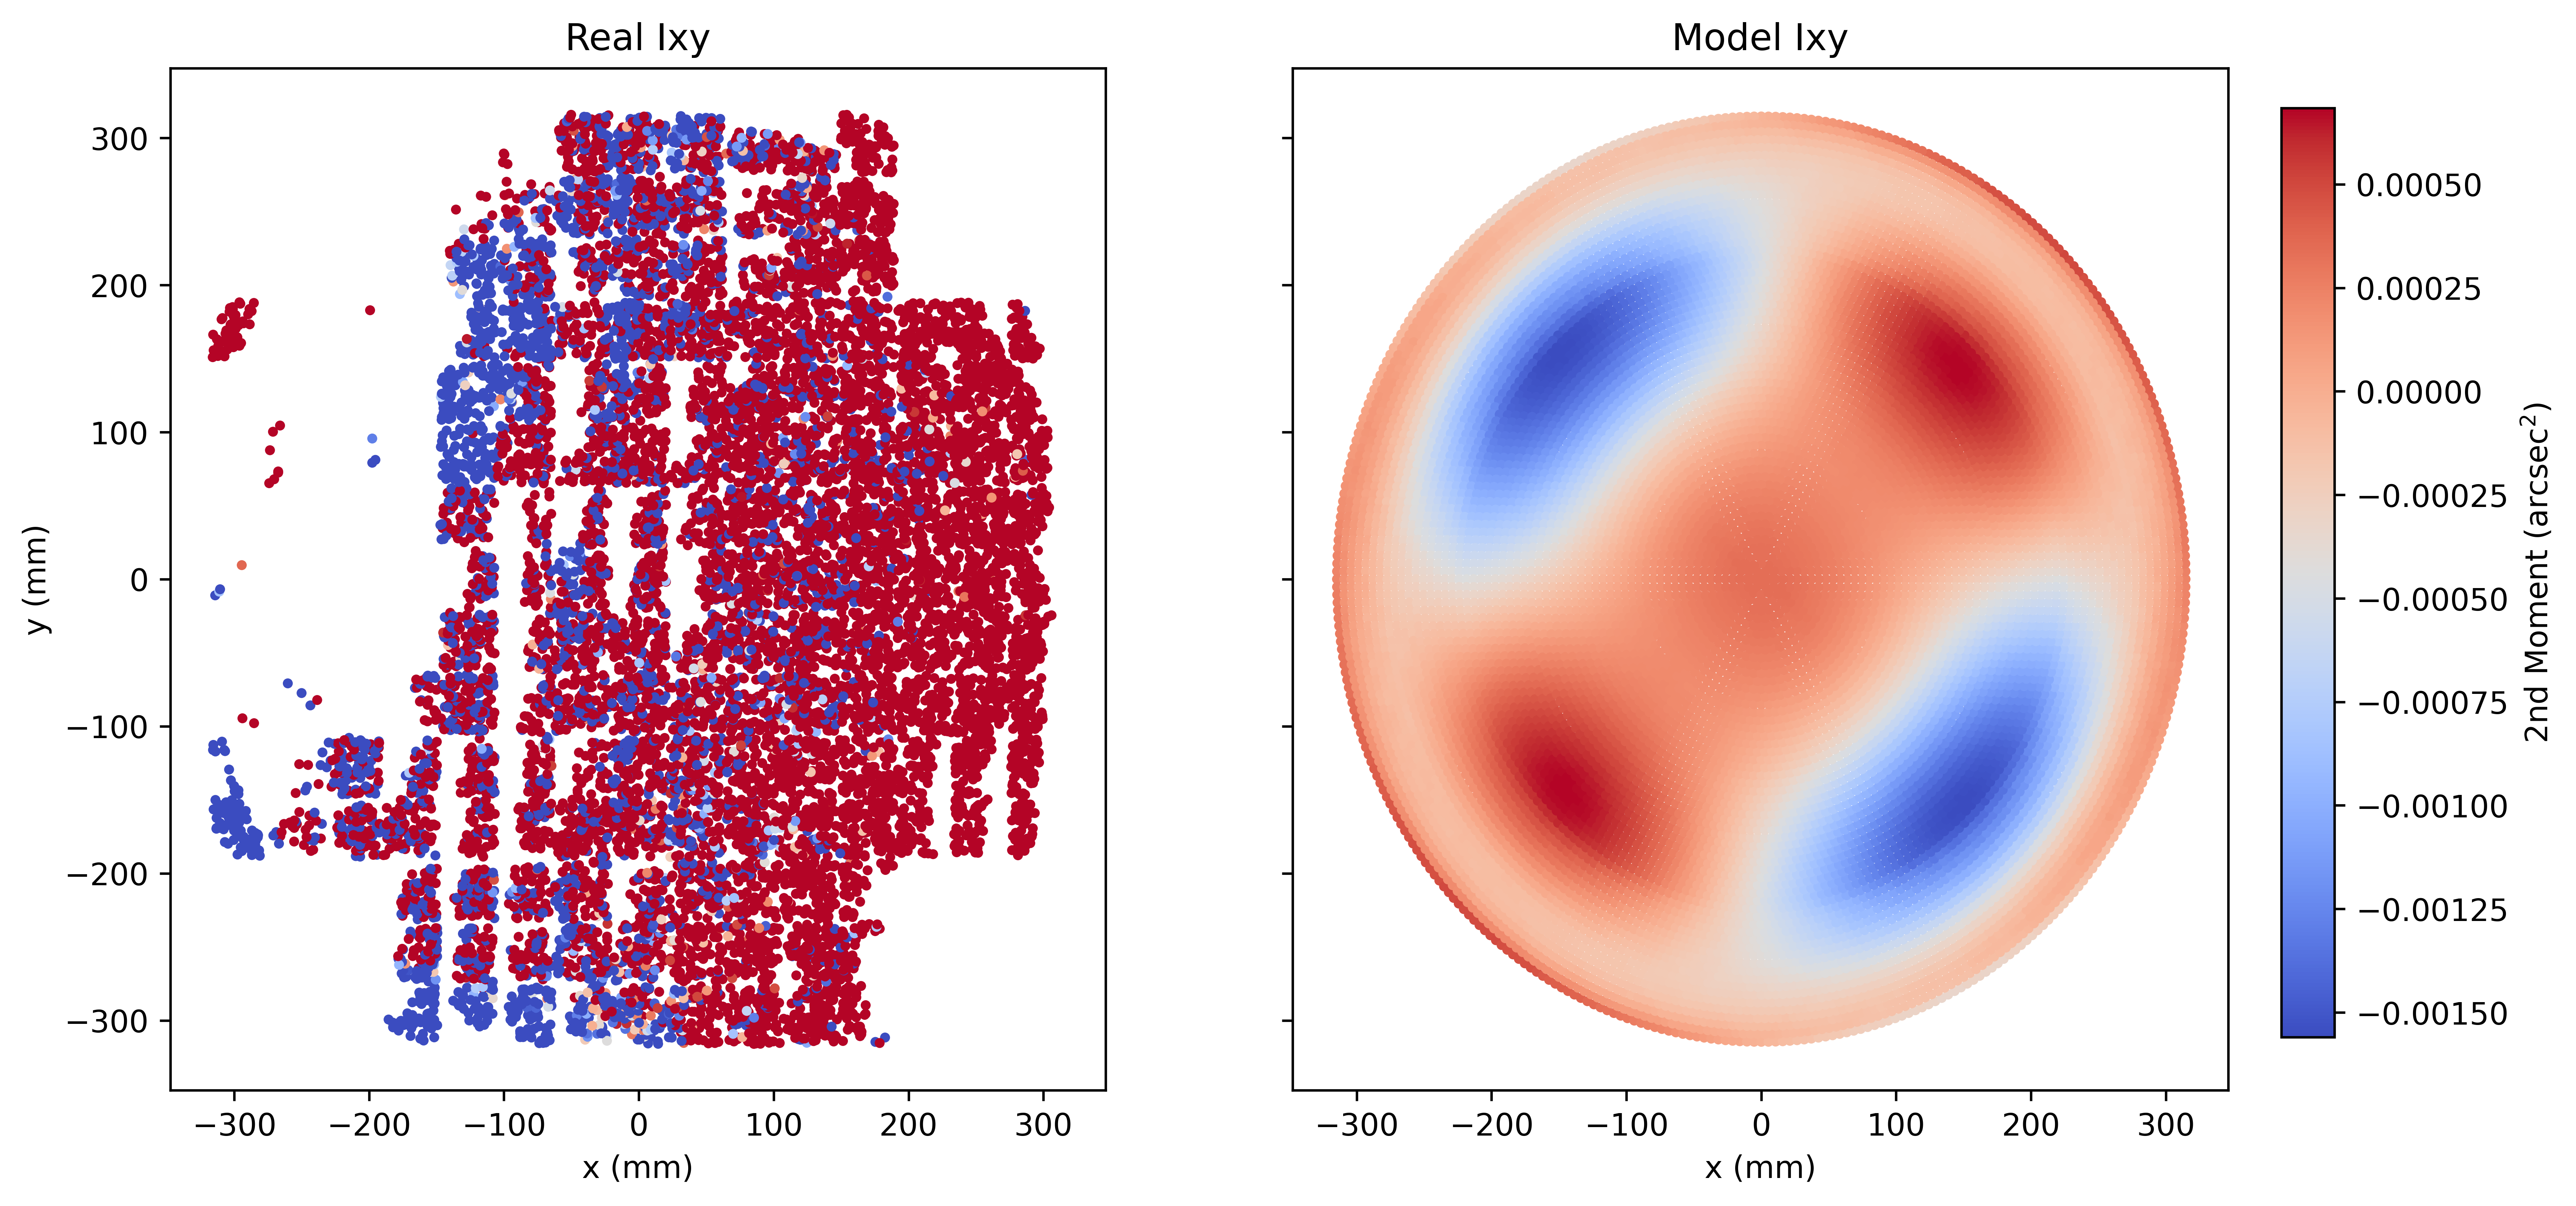
\includegraphics[width=1.0\linewidth]{2025041700635_M2_B1.png}
    \caption{Comparison between the on-sky second moment information measured using the PSF information from stars on the in-focus image and the modeled image built using \texttt{StarSharp}. This data is for the M2B1 bending mode and has a \texttt{seqnum} of 2025041700635.}
    \label{fig:example_image}
\end{figure}

The exposures for this investigation were examined by eye and formatted into an \texttt{astropy} \texttt{Table} object. 
Columns of the \texttt{Table} object consisted of information pulled out of the \texttt{ConsDB} and ASDF files built with metadata from the Butler.
This formatting allowed us to easily index the observing conditions for each set of exposures and compare between images where the expected second moment patterns were visible and those were it was not. 
Some of this data is reflected in Figure \ref{fig:conditions}, where we can see that there is not any signification correlation between the observing conditions and the visibility of the second moment patterns. 
Seeing measurements recorded by the DIMM, wind speeds, or even the total PSF do not seem to influence the visibility of these patterns. 

\begin{figure}
    \centering
    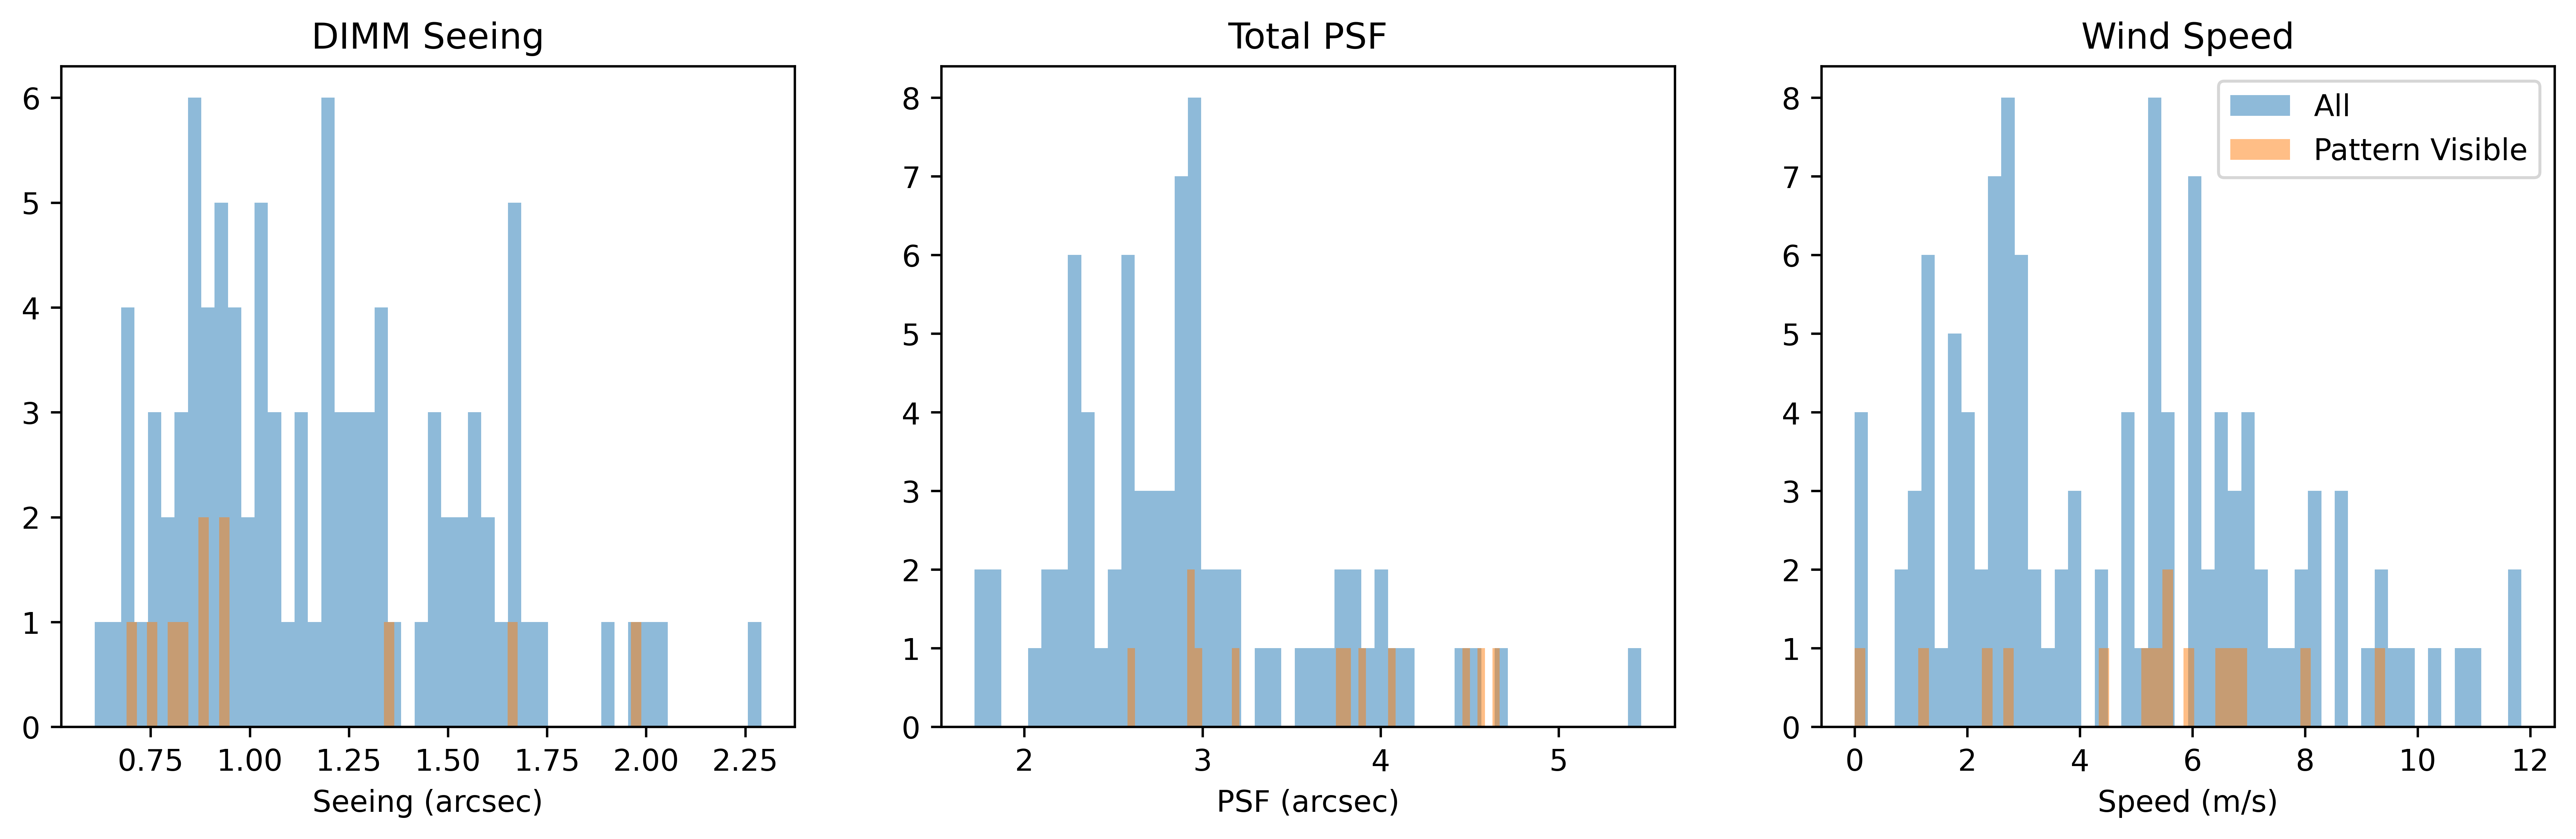
\includegraphics[width=1.0\linewidth]{multiplot.png}
    \caption{Comparisons between the observing conditions of exposures where the expected patterns were visible to the rest of the data. }
    \label{fig:conditions}
\end{figure}

An original consideration to explain why the ellipticity pattern did not seem to be recoverable in the on-sky images was a result of unpredictable behavior in the upper atmosphere not adequately represented by DIMM measurements.
However, this would have been captured by the total PSF which also showed no relationship to pattern visibility. 

While Figure \ref{fig:example_image} is an instance where the expected ellipticity pattern is not visible, 15 exposures were flagged as matching the \texttt{StarSharp} model. Figure \ref{fig:visible} is an example of this match. 

\begin{figure}
    \centering
    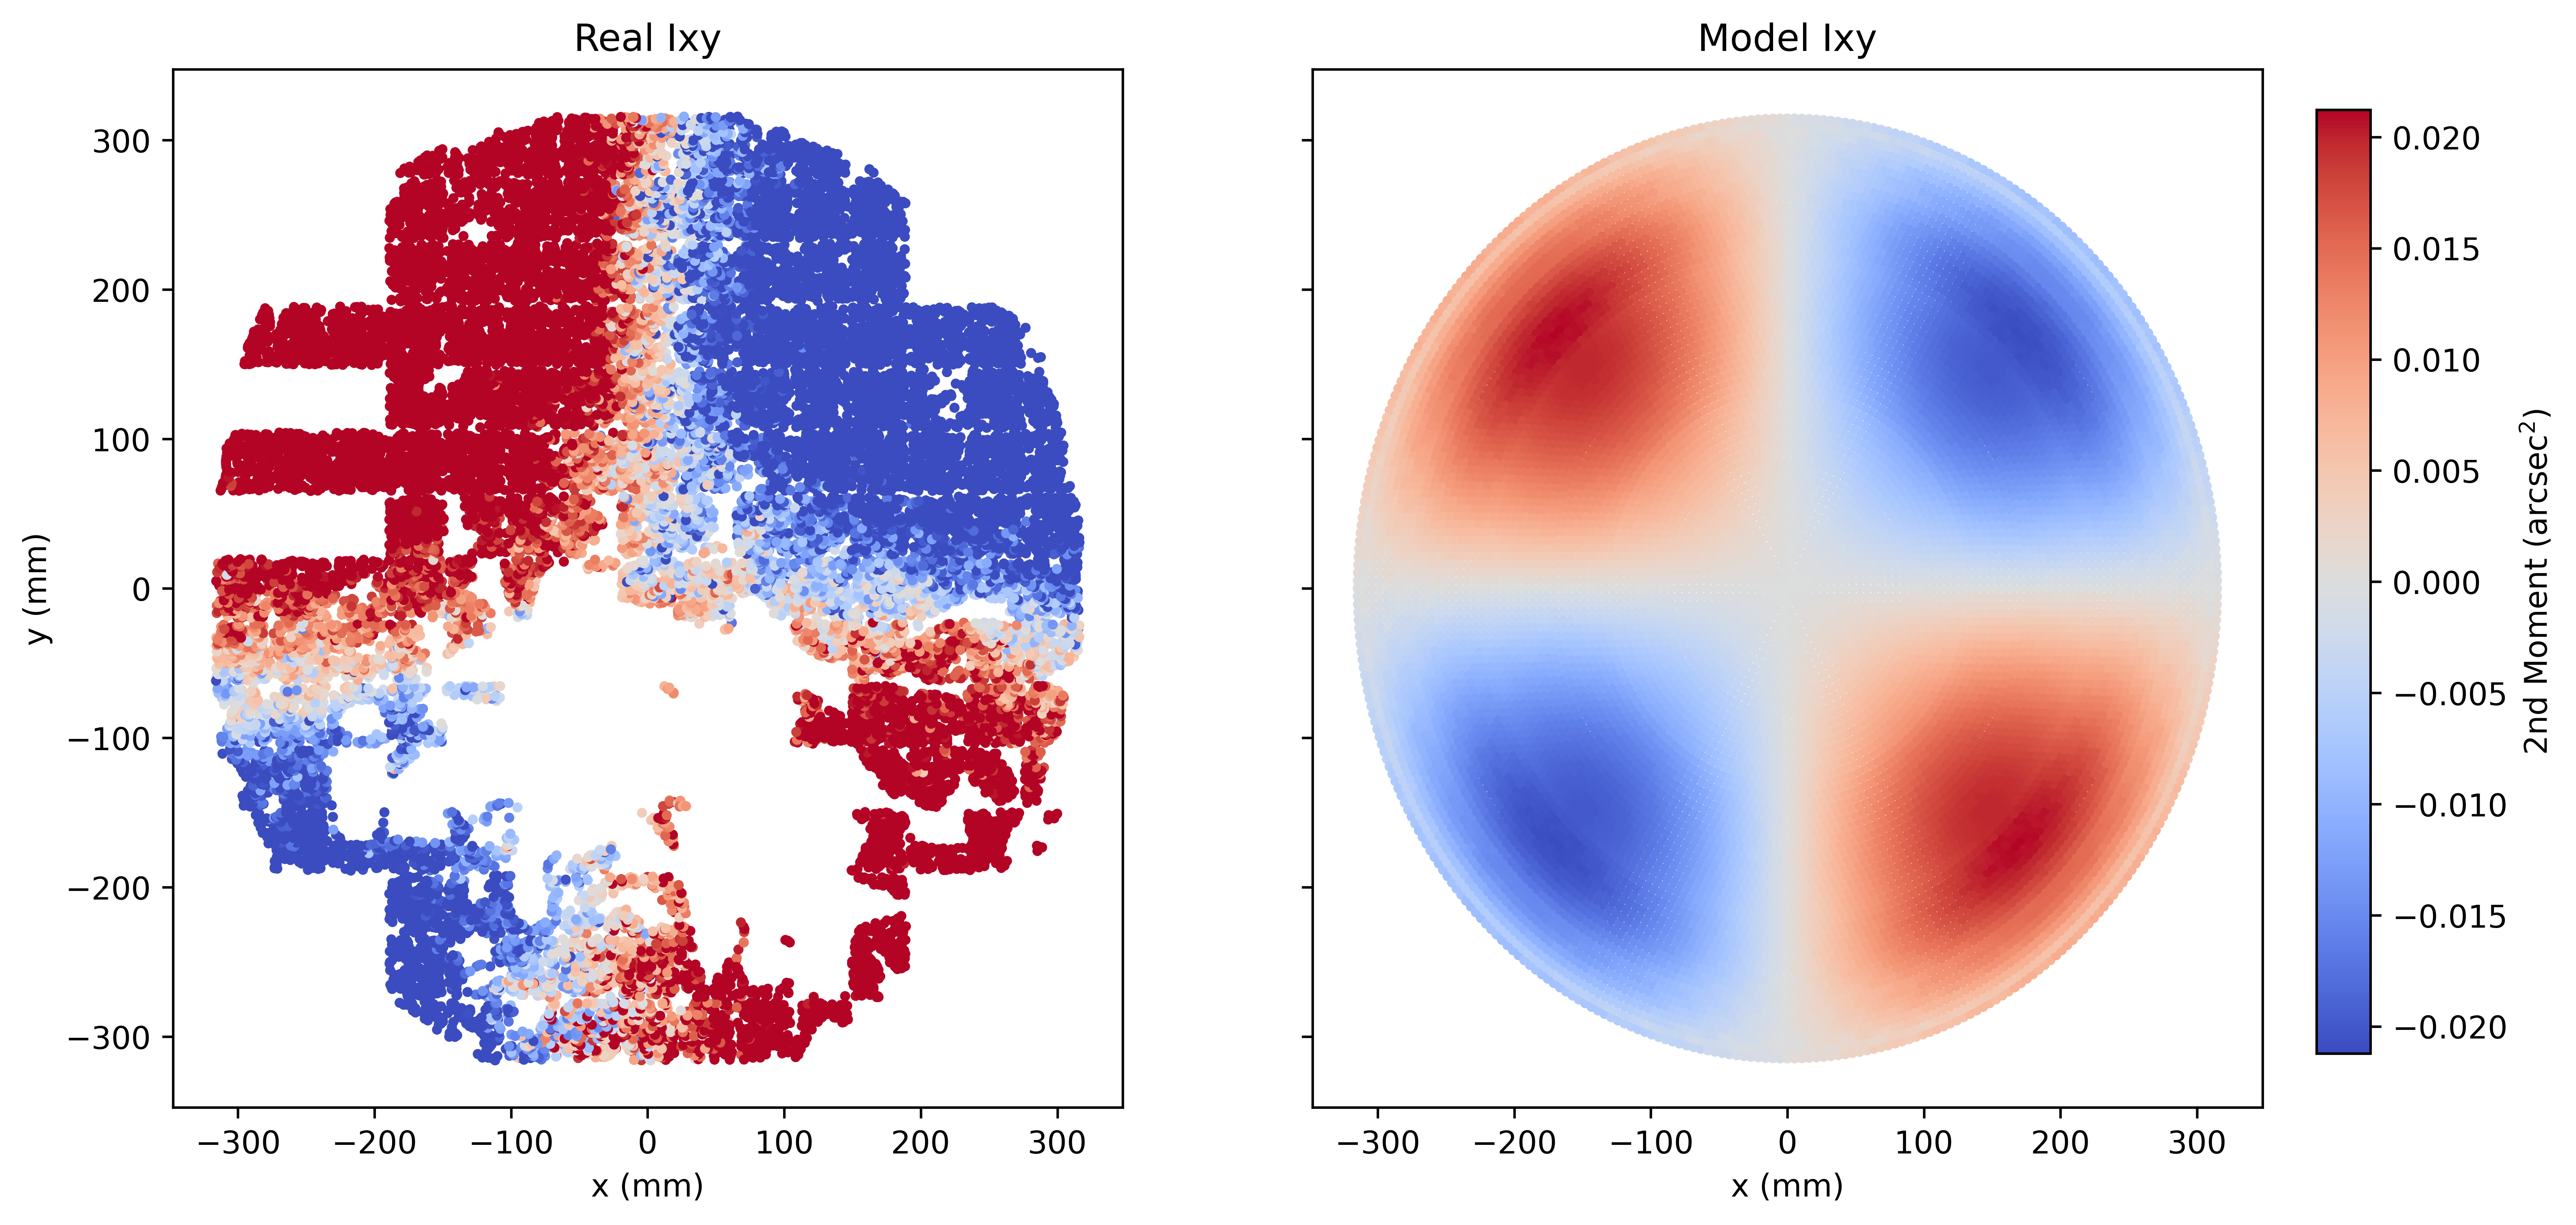
\includegraphics[width=1.0\linewidth]{2025042000586_Cam_z.png}
    \caption{Comparison between the on-sky second moment information for an exposure where the expected pattern from \texttt{StarSharp} is recoverable in the image. This exposure is manipulating the Cam-$z$ hexapod and has a \texttt{seqnum} of 2025042000586.}
    \label{fig:visible}
\end{figure}

While no correlation to the observing conditions could be established in the pattern-visible exposures, it was noted that exposures where the pattern \textit{is} visible are almost exclusively hexapod degrees of freedom as opposed to bending modes. 
This was the only real identifiable trend, as airmass, atmospheric pressure, and exposure time all also failed to show any relationship to pattern visibility.  

\section{Results and Conclusion}

Only 12.8\% of the images reflected the expected pattern for the manipulated degree of freedom. 
Initially, the hypothesis for this result was that the observing conditions and atmosphere would dominate any contribution from the degrees of freedom and the patterns might only be visible in the clearest exposures. 
However, due to the lack of relationship to any of the observing conditions, it can be concluded that the lack of pattern visibility is not a result of being dominated or masked by atmospheric conditions.
Rather, the reason for the 


The modeled ellipticity value integrated into Rubin TV rarely agrees with the measured on-sky ellipticity value, probably also due to the discrepancy of the initial conditions assumption. 


\clearpage

\appendix

\section{Acknowledgements}

This material is based upon work supported in part by the National Science Foundation through Cooperative Agreements AST-1258333 and AST-2241526 and Cooperative Support Agreements AST-1202910 and AST-2211468 managed by the Association of Universities for Research in Astronomy (AURA), and the Department of Energy under Contract No.\ DE-AC02-76SF00515 with the SLAC National Accelerator Laboratory managed by Stanford University.
Additional Rubin Observatory funding comes from private donations, grants to universities, and in-kind support from LSST-DA Institutional Members.

% https://lsst-texmf.lsst.io/lsstdoc.html#bibliographies
\section{References} \label{sec:bib}
\renewcommand{\refname}{} % Suppress default Bibliography section
\bibliography{local,lsst,lsst-dm,refs_ads,refs,books}

\clearpage

% Make sure lsst-texmf/bin/generateAcronyms.py is in your path
\section{Acronyms} \label{sec:acronyms}
\input{acronyms.tex}

\end{document}
